\subsection{Subsection Title Introduction}
This document holds the template format for all DBF related documents. This LateX project can be imported from the AIAA/Documentation folder in the official google drive. You'll need to sign to your google account using your hawk email in and have access to the AIAA drive. You can find the PDF files in our official website in the \href{https://sites.google.com/iit.edu/aiaaiit/more/resources?authuser=0}{Resources} page. 

1. Make sure that the dbf.cls, bibtex.bib, abbreviations.tex and  cover.tex are included in the folder. Try not to modify those files unless absolutely necessary. Your sections folder holds all the files you actually write content in. Try to use one files for each section and add as many as you want. Those will show up as long as you reference them each in the main.tex file. 

There should be an Images folder with two logo pictures, and a cover.png it is to be used as well. The main center cover (center\_logo.png) and another for the top left header (logo\_header.png) should be included in the Images folder. Make sure you images files are aligned with their label tag when you insert them. This let's you keep your files organised and your codes will be easier to debug. 

2. Additionally this document will show you what the tables, cites and figures will look like in the format as part of the content. Most of the contents include comments of what they, so try to read them and note them.  

3. \textit{\textbf{First Cover Page:}} Always check and rename the Title of the documentation, the top header description (put your subteam name) and update the date. 

4. \textit{\textbf{Second Page:}} Check the Authors first and last name, hawk email and IIT major department, role and year. Update published date.

5. \textit{\textbf{Third Page:}}The table of contents, acronyms, and references will be added as long as you add them to your document. They are clickable hyper-links rest assured. Red color usually means a hyperlink, black and bold text is referenced. (be it website, email, labels).

6. Finally remember to save always. And you can undo to last action if you get any compiling errors. contact any of the authors mentioned above for any of assistance or updates. 

\subsection{Citation and Links}
/*** Example of how to site an article from NASA as reference is here \cite{CLSI}.***/  Notice the reference is added to the bibtex.bib file first hand. You can do this by copying the reference in latex format from any online ref sites then paste it to the bibtex.bib. Then use the $\backslash$cite\{ref-name\} command to cite your reference. It will pop the names once you start the cite command.

/**Example of setting up hyperlinks. You can download XFLR5 by going to  \href{http://www.xflr5.tech/xflr5.htm}{www.xflr5.tech}.**/

\subsection{Equations}
/**sample Equation Formatting**/\\ %delet or comment this later
Equation Title, Book ref if possible with equation number in the book (e.g 5.9 in the book). You can refer to any equation by it's label name. For example: Equation \ref{eq:1} is used to calculate the Thrust to Weight Ratio.
\begin{equation} 
\label{eq:1}
    \frac{W}{S} = TOP \sigma C_{L,TO} \frac{T}{W} %put equation here and latex will label it
\end{equation}

Examples: \\
For Landing Distance, Raymer 5.11 provides equation \ref{eq:2} to compute the value as:
\begin{equation}
\label{eq:2}
    S_{landing} = 80 \frac{W}{S}\frac{1}{\sigma C_{L,max}} + S_a
\end{equation}

Another Example Wing Loading with Maximum Prop Range, Raymer 5.13 equation \ref{eq:3}
\begin{equation}
\label{eq:3}
    \frac{W}{S} = q \sqrt{\pi S_{ref} e C_{D0}}
\end{equation}

You can also reference an equation inserted in another page. In Introduction section \ref{s:in} on page \pageref{eq:1} an example of equation was presented. Equation \ref{eq:4} is a continuation of that on Wing Loading with Maximum Jet Range derived in Raymer 5.14. 
\begin{equation}
\label{eq:4}
    W/S = q \sqrt{\pi S_{ref} e C_{D0}/3}
\end{equation}
\subsection{Tables}
/**Example of table you can use depending the context**/
        \begin{at}{Fin Configuration Options from Solver}{tab:finsolve}{rCCR}
            $\alpha_\text{fin}$ [deg] & Tension [lbf] & $\theta$ [deg] & $x_{cable}/x_{fin}$ [--] \\
            $-5.0$ & $2.71$ & $23.2$ & $-0.061$\\
            $-2.0$ & $2.69$ & $22.3$ & $-0.020$\\
            $0.0$ & $2.68$ & $21.9$ & $0.000$\\
            $2.0$ & $2.67$ & $21.5$ & $0.021$\\
            $5.0$ & $2.66$ & $20.6$ & $0.070$\\
        \end{at}
/**Another Example of Table we can use**/ \\
You can change the row color shading scale from 10-100\% in the argument. Here's a table with 30\% gray color shading in alternating row. You can also try another type of color and shading scale as well. \\
        \begin{at}{Fin Configuration Options from Solver}{tab:finsolve}{rCCR}
            $\alpha_\text{fin}$ [deg] & Tension [lbf] & $\theta$ [deg] & $x_{cable}/x_{fin}$ [--]\\
        \rowcolor{gray!30} $-5.0$ & $2.71$ & $23.2$ & $-0.061$\\
                           $-2.0$ & $2.69$ & $22.3$ & $-0.020$\\
        \rowcolor{gray!30} $0.0$ & $2.68$ & $21.9$ & $0.000$\\
                           $2.0$ & $2.67$ & $21.5$ & $0.021$\\
        \rowcolor{gray!30} $5.0$ & $2.66$ & $20.6$ & $0.070$\\
        \end{at}

\subsubsection{Tables with custom environment tag}
/**Another Example of Table we can use with custom row color. Use can pass the 'atb' argument to give the first column it's own custom color. It will be a gray fill with a white color text. Notice the atb is an environment argument defined in the css. **/
        \begin{atb}{Landing Gear Configuration Matrix}{tab:gearconfig}{l *{7}{C}}
            \makebox[.2\linewidth]{\centering Criteria} & Weight & Tricycle & Tail-Dragger \\
            Handling Characteristics & 30 & 2 & 1 \\
            Deployment Reliability & 25 & 2 & 1 \\
            Ease of Manufacturing & 20 & 2 & 1 \\
            Drag & 15 & 1 & 2 \\
            Weight & 10 & 1 & 2 \\\hlineB{2.5}
            \textbf{Total} & 100 & 175 & 125
        \end{atb}
        %
/** Another table combination of all of the above **/
 {
        \begin{atb}{Fuselage Selection Matrix}{tab:fuseselect}{l *{4}{C}}
            \makebox[.2\linewidth]{\centering Criteria} & Weight & Single Fuselage & Twin-Fuselage  \\
            Lift & 25 & 2 & 1  \\
            Weight & \rowcolor{gray!20} 20 & 2 & 1  \\
            Payload Capacity &  20 & 1 & 2  \\
            Drag & \rowcolor{gray!20} 20 & 2 & 1  \\
            Stability & 10 & 1 & 2  \\
            Ease of Manufacture & \rowcolor{gray!20} 5 & 2 & 1 \\
            \hlineB{2.5}
            \textbf{Total} & 100 & 170 & 130  \\
        \end{atb}}
        %

\subsubsection{Tables with different cell colors}
/** You can combine cell colors to create something like \ref{tab:sensor_ffs}**/. Those are handy whenever you want to do a quick selection matrix and such based on cell color.  
\begin{table}[H]
    \caption{Sensor Flip Flops}
    \label{tab:sensor_ffs}
    \begin{subtable}{.32\textwidth}
        \caption{D-Flip-Flop A}
        \vspace{-.5em}
        \centering
        \begin{tabular}{*{5}{c}}
            \cellcolor{iitred}\color{white}DA & \mc{4}{c}{\cellcolor{iitred}\color{white}CI}\\
            \cellcolor{iitred}\color{white}AB & \cellcolor{iitred}\color{white}00 & \cellcolor{iitred}\color{white}01 & \cellcolor{iitred}\color{white}11 & \cellcolor{iitred}\color{white}10\\
            \cellcolor{iitgray}\color{white}00 & \cellcolor{yellow}1 & \cellcolor{orange}1 & \cellcolor{orange}1 & \cellcolor{yellow}1\\
            \cellcolor{iitgray}\color{white}01 & \cellcolor{yellow}1 & 0 & x & \cellcolor{yellow}x\\
            \cellcolor{iitgray}\color{white}11 & x & x & x & x\\
            \cellcolor{iitgray}\color{white}10 & 0 & \cellcolor{orange}1 & \cellcolor{orange}x & x\\
        \end{tabular}
    \end{subtable}
    \begin{subtable}{.32\textwidth}
        \caption{D-Flip-Flop B}
        \vspace{-.5em}
        \centering
        \begin{tabular}{*{5}{c}}
            \cellcolor{iitred}\color{white}DB & \mc{4}{c}{\cellcolor{iitred}\color{white}CI}\\
            \cellcolor{iitred}\color{white}AB & \cellcolor{iitred}\color{white}00 & \cellcolor{iitred}\color{white}01 & \cellcolor{iitred}\color{white}11 & \cellcolor{iitred}\color{white}10\\
            \cellcolor{iitgray}\color{white}00 & \cellcolor{yellow}1 & \cellcolor{yellow}1 & \cellcolor{yellow}1 & \cellcolor{yellow}1\\
            \cellcolor{iitgray}\color{white}01 & 0 & 0 & x & x\\
            \cellcolor{iitgray}\color{white}11 & x & x & x & x\\
            \cellcolor{iitgray}\color{white}10 & \cellcolor{yellow}1 & \cellcolor{yellow}1 & \cellcolor{yellow}x & \cellcolor{yellow}x\\
        \end{tabular}
    \end{subtable}
    \begin{subtable}{.32\textwidth}
        \caption{D-Flip-Flop C}
        \vspace{-.5em}
        \centering
        \begin{tabular}{*{5}{c}}
            \cellcolor{iitred}\color{white}DC & \mc{4}{c}{\cellcolor{iitred}\color{white}CI}\\
            \cellcolor{iitred}\color{white}AB & \cellcolor{iitred}\color{white}00 & \cellcolor{iitred}\color{white}01 & \cellcolor{iitred}\color{white}11 & \cellcolor{iitred}\color{white}10\\
            \cellcolor{iitgray}\color{white}00 & \cellcolor{yellow}1 & \cellcolor{orange}1 & \cellcolor{orange}1 & 0\\
            \cellcolor{iitgray}\color{white}01 & \cellcolor{yellow}1 & 0 & x & x\\
            \cellcolor{iitgray}\color{white}11 & \cellcolor{yellow}x & x & x & x\\
            \cellcolor{iitgray}\color{white}10 & \cellcolor{yellow}1 & \cellcolor{orange}1 & \cellcolor{orange}x & x\\
        \end{tabular}
    \end{subtable}
\end{table}

%%%%%%%%%%%%%%

\subsubsection{Risk Tables}
/***Simple risk table indicator**/
Table \ref{Tab:rcg} is whenever we need for matching the cell color to it's cell value or description. In this case risk tables are easier to indicate. For example, Bright red is a high probability and extremely severe. \\
\begin{table}[hbt!]
\caption{Risk Color-grading}
\label{Tab:rcg}
\centering
\resizebox{\textwidth}{!}{%
\begin{tabular}{|c|ccccc|}
\hline
& \multicolumn{5}{c|}{\textbf{Risk Severity}} \\ \hline
& \multicolumn{1}{c|}{}               & \multicolumn{1}{c|}{Catastrophic (4)}           & \multicolumn{1}{c|}{Major (3)}                  & \multicolumn{1}{c|}{Minor (2)}                  & Negligible (1)             \\ \cline{2-6} 
 & \multicolumn{1}{c|}{Frequent (A)}   & \multicolumn{1}{c|}{\cellcolor[HTML]{FE2200}A4} & \multicolumn{1}{c|}{\cellcolor[HTML]{FD6864}A3} & \multicolumn{1}{c|}{\cellcolor[HTML]{FFCC67}A2} & \cellcolor[HTML]{FFFC9E}A1 \\ \cline{2-6} 
& \multicolumn{1}{c|}{Occasional (B)} & \multicolumn{1}{c|}{\cellcolor[HTML]{FD6864}B4} & \multicolumn{1}{c|}{\cellcolor[HTML]{FFCC67}B3} & \multicolumn{1}{c|}{\cellcolor[HTML]{FFCC67}B2} & \cellcolor[HTML]{B0D9AF}B1 \\ \cline{2-6} 
\multirow{-4}{*}{\textbf{\begin{tabular}[c]{@{}c@{}}Risk \\ Probability\end{tabular}}} & \multicolumn{1}{c|}{Improbable (C)} & \multicolumn{1}{c|}{\cellcolor[HTML]{FFFC9E}C4} & \multicolumn{1}{c|}{\cellcolor[HTML]{FFCC67}C3} & \multicolumn{1}{c|}{\cellcolor[HTML]{B0D9AF}C2} & \cellcolor[HTML]{9AD698}C1 \\ \hline
\end{tabular}
}
\end{table}

\vspace{1cm}
/***Expanded risk table indicator**/\\

\begin{table}[hbt!]
\caption{Mission Risks }
\centering
\begin{tabular}{lll}
\rowcolor[HTML]{C0C0C0} 
Main Risks anticipated                                 & Mitigation Plan Utilized                                                                          & Value \\
\cellcolor[HTML]{FD6864}B4 - Space Debris & \begin{tabular}[c]{@{}l@{}}Use onboard active tracking software\\ maneuvering\end{tabular}        & 4     \\
\cellcolor[HTML]{FD6864}A3 - Radiation         & \begin{tabular}[c]{@{}l@{}}Use a double wall bumper. Cheaper\\ than carbon nanotube components\end{tabular} & 3 \\
\cellcolor[HTML]{FFCC67}A2 - Thermal      & \begin{tabular}[c]{@{}l@{}}Silver-coated teflon instead of optical\\ solar reflector\end{tabular} & 2     \\
\cellcolor[HTML]{F2C875}B3 - Cost         & \begin{tabular}[c]{@{}l@{}}Compared components over several\\ commercial sites\end{tabular}       & 3     \\
\cellcolor[HTML]{F2C875}B2 - Launching Risks   & \begin{tabular}[c]{@{}l@{}}Selected Falcon heavy as the safest\\ possible option\end{tabular}               & 2 \\
\cellcolor[HTML]{FFFC9E}C4 - Foreign Satellite & \begin{tabular}[c]{@{}l@{}}Effective communication using ARM\\ Cortex with other satellites\end{tabular}    & 4 \\
\cellcolor[HTML]{FFFC9E}C3 - Solar Flare       & \begin{tabular}[c]{@{}l@{}}Course correction using BiSon64\\ and 2U propulsion for ADCS\end{tabular}        & 3
\end{tabular}
\label{Tab:mra}
\end{table}

\subsection{Figures}
/**Example of figure with a width of 10cm is shown here. You can specity the width and height too as you'd like. **/ \\
\begin{figure}[H]
        \centering
        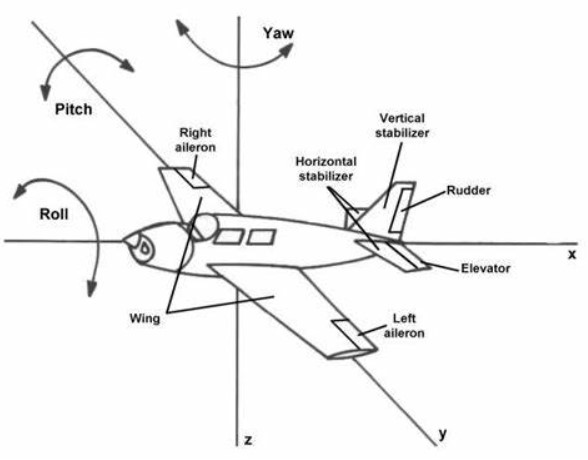
\includegraphics[width=10cm]{Images/Control surfaces.jpg}
        \caption{Label your figure here e.g for the NACA 2412.}
        \label{fig:my_label}
    \end{figure}

/**Another Example of double figures**/ \\
 \begin{figure}[H]
            \centering
            \begin{subfigure}{.49\textwidth}
                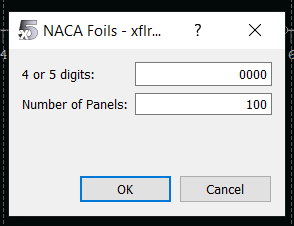
\includegraphics[width=\textwidth]{Images/NACA foils.PNG}
                \caption{$C_l$ vs $\alpha$}
            \end{subfigure}
            \hspace{\fill}
            \begin{subfigure}{.49\textwidth}
                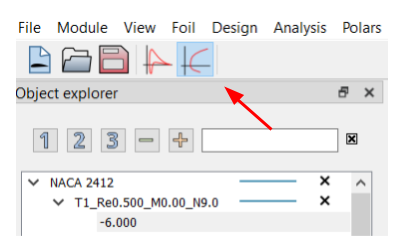
\includegraphics[width=\textwidth]{Images/polar view.png}
                \caption{$L/D$ vs $\alpha$}
            \end{subfigure}
            \caption{Airfoil Aerodynamic Properties @ Re $= 300,000$}
            \label{fig:foilprops}
        \end{figure}

% \newpage
\subsection{Shapes and Graphs}

/**Example graphs and shapes**/\\

    \begin{figure}[!ht]
        \centering
        \begin{tikzpicture}[ultra thick, circle, color=white, -{Latex[round,width=10,length=10]}]
            \node [fill=iitred] at (0,0) (000) {000};
            \node [fill=iitred] at (3,0) (100) {100};
            \node [fill=iitred] at (6,0) (010) {010};
            \node [fill=iitred] at (9,0) (001) {001};
            \node [fill=iitred] at (4.5,-2) (111) {111};
            
            \draw[color=black] (000.east)+(.1,0) -- (100.west) node[midway,fill=white,inner sep=0] {\large 1};
            \draw[color=black] (100.east)+(.1,0) -- (010.west) node[midway,fill=white,inner sep=0] {\large 1};
            \draw[color=black] (010.east)+(.1,0) -- (001.west) node[midway,fill=white,inner sep=0] {\large 1};
            \draw[color=black] (001.north)+(0,.1) |- ++(-3,.5) -- ++(-3,0) node[midway,fill=white,inner sep=0] {\large 1} -| (000.north);
            \draw[color=black] (000.south)+(0,-.1) -- ++(0,-1.5) -- (111.west) node[midway,fill=white,inner sep=0] {\large 0};
            \draw[color=black] (100.south east)+(.05,-.1) -- (111.north west) node[midway,fill=white,inner sep=0] {\large 0};
            \draw[color=black] (010.south west)+(-.05,-.1) -- (111.north east) node[midway,fill=white,inner sep=0] {\large 0};
            \draw[color=black] (001.south)+(0,-.1) -- ++(0,-1.5) -- (111.east) node[midway,fill=white,inner sep=0] {\large 0};
            \draw[color=black] (111.south)+(0,-.1) -- ++(0,-.5) -- ++(-5.75,0) node[midway,fill=white,inner sep=0] {\large 0, 1} |- (000.west);
        \end{tikzpicture}
        \vspace{-1em}
        \caption{Sensor Pod Finite State Machine Diagram}
        \label{fig:sensor_fsm}
    \end{figure} 

%%%%%%%%%%%%%%
\vspace{1.5cm}
\subsubsection{Shapes}
/**Charts**/\\
\begin{figure}[!ht]
        \centering
        \renewcommand{\baselinestretch}{.7}
        \begin{tikzpicture}[thick, rectangle,rounded corners=5pt,align=center,color=white,minimum width=1.1in,minimum height=.5in]
            \node[fill=iitred] at (1,4.25) (advisor) {\footnotesize First Last\\\footnotesize Faculty Advisor};
            \node[fill=iitred] at (5,4.25) (mikel) {\footnotesize First Last\\\footnotesize Additional Advisor (if any)};
            \node[fill=iitgray] at (1,2.25) (pm) {\footnotesize First Last\\\footnotesize Project Manager};
            \node[fill=iitgray] at (5,2.25) (le) {\footnotesize First Last\\\footnotesize Lead Engineer};
            \node[fill=iitred] at (0,0) (aero1) {\footnotesize First Last\\\footnotesize Aerodynamics\\\footnotesize (Wing)};
            \node[fill=iitred] at (0,-1.5) (aero2) {\footnotesize First Last\\\footnotesize Aerodynamics\\\footnotesize (Co-Lead if any)};
            \node[fill=iitred] at (3.5,0) (struc) {\footnotesize First Last\\\footnotesize Structures};
            \node[fill=iitred] at (6.5,0) (prop) {\footnotesize First Last \\\footnotesize Propulsion};
            
            \draw[color=black] (advisor.south) -- (pm.north);
            \draw[color=black] (mikel.south) -- (le.north);
            \draw[color=black] (pm.south) |- ++(.75,-.5) node[rounded corners]{} -- ++(0,-1) |- (aero1.east);
            \draw[color=black] (1.75,0) |- (aero2.east);
            \draw[color=black] (1.25,1.1) -| (le.south);
            \draw[color=black] (struc.north) |- (2,1.1) -| (prop.north);
            \draw[color=black] (struc.north) |- (4,1.1);
            \draw[color=black] (2,1.1) -| (1.75,.5);
            \draw[color=black] (le.south) |- ++(.5,-.5);
            \draw[color=black] (pm.east) -- (le.west);
        \end{tikzpicture}
        \caption{Team Structure and Leaders}
        \label{fig:org_chart}
        \vspace{-1em}
    \end{figure} 
    
%%%%%%%%%%%%%%%%%%%%%%%%  

\subsubsection{Flowcharts}
/**Additional flowchart style**/
\tikzstyle{decision} = [diamond, fill=gray!50, text badly centered, node distance=3cm, inner sep=0pt]
\tikzstyle{block} = [rectangle, fill=red!37, text centered, rounded corners, minimum height=4em]
\tikzstyle{line} = [draw, -{Latex[width=5pt,length=7pt]}]
\tikzstyle{cloud} = [ellipse, fill=iitred, node distance=3cm, minimum height=2em]
\vspace{0.5cm}
\begin{figure}[H]
\caption{Mission Analysis}
    \centering
    \begin{tikzpicture}[node distance = 2cm, auto, text=black, inner sep=5pt, align=center]
        % Place nodes
        \node [block] (design) {Phase 1};
        \node [block, right of = design, node distance = 3.5cm] (manufacturing) {Phase 2};
        \node [block, right of= manufacturing, node distance = 3.5cm] (assembly) {Phase 3 };
        \node [block, right of= assembly, node distance = 3.5cm] (testing) {Analysis};
        \node [block, below of= assembly, node distance = 2cm] (feedback) {Conclusion};
        \node [block, right of= testing, node distance = 3.5cm] (final) {References};
        
        % Draw edges
        \path [line] (design) -- (manufacturing);
        \path [line] (manufacturing) -- (assembly);
        \path [line] (assembly) -- (testing);
        \path [line] (testing) |- (feedback);
        \path [line] (feedback) -| (design);
        \path [line] (testing) -- (final);
    \end{tikzpicture}
    \label{fig:manplan}
\end{figure}

\newpage
\subsection{Item lists, bullets and numbers}
/**Example of item lists to use**/
 \begin{itemize}
        \item Module $>$  Foils
        \item Foil $>$ NACA Foils
    \end{itemize}
    